\addcontentsline{toc}{section}{Overview of Lectures 2-7}
\chapter*{Overview of Lectures 2-7}
Let's see what we have in the upcoming lectures:\\

\begin{itemize}
    \item \textbf{Lecture 2: }Synchronous model. In these models, we assume that messages are delivered in a reasonable amount of time. There will be a bound $\Delta$ on the number of time steps it can elapse before that message is guaranteed to have been received. For example, for the best-case operation of the internet, the $\Delta$ is assumed somewhere near a second.\\
    The good news about the synchronous model is that it enables some pretty impressive
    SMR protocols. The main goal of Lecture 2 is to explain the design and analysis of such
    a protocol, known as the Dolev-Strong protocol (from the early 1980s). This protocol is
    for a single-shot consensus problem known as “Byzantine broadcast,” but we’ll also see in
    Lecture 2 how to reduce the SMR problem (which is the multi-shot consensus) to the Byzantine
    broadcast problem. This reduction extends the Dolev-Strong protocol to an SMR protocol
    with all the properties that we might want. What’s really extraordinary about the DolevStrong protocol is that it tolerates an arbitrarily large number of dishonest nodes. Even if
    98 out of 100 nodes are malicious and acting in cahoots, there’s nothing they can do to trick
    the remaining 2 honest nodes into getting out of sync. The disadvantage of the synchronous
    model is that its assumptions are simply too strong to provide accurate guidance for the
    design of Internet-scale protocols.
    You won’t see the Dolev-Strong protocol referenced very often in blockchain whitepapers
    and discussions, but it’s worth studying for several reasons. One, if you ever do find yourself
    in a setting where the synchronous model is appropriate (perhaps in a private network), you’ll
    know how to achieve a pretty amazing set of guarantees. Second, studying this (relatively
    simple) protocol will act as a good warm-up to more complicated protocols that we’ll see
    later (like Tendermint)—we’ll get a sense of what typical consensus protocols look like and
    how they can make use of tools such as digital signatures. Finally, it’s a famous result—
    definitely part of the distributed computing greatest hits and readers who identify as
    card-carrying computer scientists should enjoy learning how and why it works.

    \item \textbf{Lecture 3: }Synchronous model, Lecture 3 is where we see our first impossibility result which, like the one in Lecture 6, rules
    out good SMR protocols when at least 33\% of the nodes can deviate from the protocol (or in other words 67\% honest nodes are needed).
    Unlike the Lecture 6 impossibility result (for the partially synchronous model), the one here
    applies even in the (easier) synchronous model. But wait, why doesn’t this contradict the
    guarantees promised by the Dolev-Strong protocol, which hold even when almost all the
    nodes are malicious?
    This lecture drills down on a key assumption made by the Dolev-Strong protocol, typically
    called the PKI (for “public key infrastructure”) assumption. Here we're not just assuming that cryptography exists and that anybody has access to a secure digital signature scheme but we're also assuming that prior to the commencement of the protocol, all the nodes' public keys are common knowledge. The assumption is that all the
    nodes running the protocol have their own public key-private key pairs and that all nodes’
    public keys were somehow exchanged before the commencement of the protocol. In other
    words, all nodes begin the protocol with the ability to verify a signature by any other node.
    While the PKI assumption is fairly palatable in a blockchain context, it winds up being
    quite interesting to study what’s possible without it and other “trusted setup” assumptions.
    And the 33\% impossibility result of this lecture pops up already in the synchronous setting
    when there are no trusted setup assumptions. The proof of this impossibility result—due
    to Fischer-Lynch-Merritt and called the “hexagon argument,” for reasons that will become
    clear—is impressively slick. For those of you who like cool proofs, Lecture 3 is likely to be
    your favorite one of the course. Conversely, if you’re not into proofs and wanted to skip
    one of these six lectures, Lecture 3 should probably be the one. It’s a famous and enlightening
    result that belongs to the distributed computing canon (like the other impossibility results
    in the course), but it is not 100\% essential to the course’s overarching narrative.
    
    \item \textbf{Lectures 4,5: }Asynchronous model, The synchronous model allows consensus protocols with amazing guarantees (at least under
the PKI assumption) but makes assumptions that are simply too strong for protocols that
operate over the Internet. Therefore, we have no choice but to weaken our assumptions about
the underlying communication network. One natural idea is to assume nothing about the
communication network, other than the minimal property that every message is delivered
eventually. This is the idea behind the “asynchronous model”.
The good news about the asynchronous model is that, with essentially no assumptions
about the communication network, any consensus protocol with non-trivial provable guarantees in the model would automatically be impressively robust. The bad news is that this
model throws out the baby with the bathwater, in the sense that consensus is provably impossible (at least for deterministic protocols). This result, due to Fischer-Lynch-Paterson,
is perhaps the most famous impossibility result in all of distributed computing. Its proof
will be the hardest one that we’ll see in this course, and probably the hardest one in the
whole lecture series. We’ll get started on the proof in Lecture 4 (after formally defining the
asynchronous model) and finish it off in Lecture 5.
The key takeaway from the FLP impossibility result is that the asynchronous model simply doesn’t make enough assumptions. The point of a model is to help us brainstorm about the space of protocols and hopefully identify some that work well in both theory and
practice. With no good (deterministic) protocols in this model, there’s not much brainstorming to be done! The FLP impossibility result thus completes the justification for introducing
a third model (the partially synchronous model) in Lecture 6. While slightly less natural than
the synchronous or asynchronous model, it acts as a sweet spot between the two, with assumptions that are weak enough to be relevant to Internet-scale protocols and strong enough
so that practical consensus protocols with provable guarantees actually exist.

    \item \textbf{Lecture 6: } This lecture will be about partially synchronous model. The main idea is to look at the operation of a protocol in 2 different phases: 1- Normal operations where messages get delivered in a reasonable amount of time and 2- Attack mode: Situations where there's big network outages and attacks. The Synchronous model says that you don't want to break too badly under attack and that you recover quickly when the attack ends. The partially synchronous model is quite important in the analysis of blockchain protocols. This lecture  introduces the partially synchronous model as a sweet spot between the
    synchronous and asynchronous models, proves that consensus is impossible in this
    model when more than 33\% of the nodes can deviate from the protocol, and compares
    these results to a famous principle from distributed systems, the CAP theorem. 
    \item \textbf{Lecture 7: } We're going to talk about the Tendermint protocol. In this lecture, we're mainly focusing on principles rather than protocols, but lecture 7 will be about a specific blockchain protocol that's used in the real world and we will discuss its provable guarantees which include Consistency and "eventual" Liveness. Through these proofs not only do we understand how Tendermint works, but also why it works the way it does.
\end{itemize}

If we look at the main layer one of the protocols we can see that most of them fall into two camps:

\begin{enumerate}
    \item \textbf{BFT-type protocols} We will refer to blockchain protocols that resemble the consensus
    protocols from the 1980s and 1990s (like Tendermint) as BFT-type protocols. (Here BFT
    stands for “Byzantine fault tolerant.”) Several of the major “layer-1” networks use BFTtype blockchains, including Solana, Terra, Cosmos, and Algorand. When Facebook/Meta
    was considering rolling out its own blockchain (for the Diem cryptocurrency), they were
    planning to base it on a BFT-type protocol called HotStuff. Thus, This course prepares
    you well to understand how these BFT-type blockchain protocols work. In this type, failure is mostly caused by progress stalls (no new blocks are created) which happens because this type of protocol favors safety over liveness.

 \item \textbf{Longest-chain protocols} We haven't mentioned the two
    most famous blockchain protocols of them all, Bitcoin and Ethereum. These two protocols
    achieve consensus in a radically different way and are examples of longest-chain protocols.
    The idea of longest-chain consensus does not come from the classical consensus literature
    and was invented specifically for the Bitcoin protocol. (Several blockchain protocols that
    came later, including Ethereum, also adopted longest-chain consensus.
    ) Our first order
    of business after our classical consensus topics is to develop a deep understanding of
    longest-chain consensus and its pros and cons relative to BFT-type consensus. We’ll get
    started on this topic in Lecture 8. In this type(Specially for Bitcoin or Ethereum), we don't really have stopping or stalling. So the problem isn't caused by progress stalls but there's a massive rollback of a bunch of transactions in favor of an entirely different batch of transactions, due to the fact that this type of protocol favors liveness over safety.
\end{enumerate}

At the end of these lectures, you will have accomplished two really important things.
First, you’ll have mastered the basic concepts behind one of the two major design paradigms
for blockchain protocols (BFT-type protocols). Second, and possibly even more important,
you’ll be equipped with the mental model, the formal definitions, and the language to discuss,
assess, and rigorously compare different blockchain consensus protocols (including longestchain protocols and anything else that protocol designers manage to come with).\\

What's even more important to remember is the lens through which we look at these different parts of the design space and assess the different trade-offs that they're making. For example, some types of blockchain protocols favor saftey like BFT-type protocols and some favor liveness like Longest-chain protocols. So, by mastering the partially synchronous model and the impossibility results therein, we can actually know what people mean when they say one blockchain favors safety and the other favors liveness. Also, we can understand why different blockchain protocols fail in different ways.



\chapter{Byzantine Broadcast in the
Synchronous Model via the
Dolev-Strong Protocol}

\section{Recap of SMR Problem}
The goal of this lecture is to design and analysis a consensus protocol that solves the state
machine replication (SMR) problem under a strong assumption about the underlying communication network (known as the “synchronous model” assumption), meaning that the
protocol is guaranteed to satisfy both consistency and liveness. Recall the definition of the
SMR problem from Lecture 1:\\

\begin{enumerate}
    \item There is a set of nodes responsible for running a consensus protocol, and a set of clients
who may submit “transactions” to one or more of the nodes. 

    \item So what are nodes doing besides just
receiving and transactions from clients?
Each node is
responsible for maintaining a locally
stored history. Each node maintains a local append-only data structure—an ordered list of transactions that only grows over time—which we’ll call its history.

\end{enumerate}

For us, “clients” represent users of a blockchain protocol, “nodes” refer to the machines
actually running the protocol, and a “transaction” would be something like a cryptocurrency
transfer or a smart contract function call.

As we said in the previous lecture, order is very important to us. 
For example, if
we think about two transactions that are
currency payments both trying to spend
the same coins(a sort of an intended
double spend attack perhaps), it really
matters which of those two transactions
comes first in the history. The first
transaction will succeed and the coins
will be spent. When the second
transaction comes along, there are no such coins available and that transaction
would fail. So they maintain the
transactions that have been executed
along with the order in which they have
been executed.\\

Recall also that a protocol is, informally, a piece of code that is to be run by each of the
nodes to manage the local computation and communication by the node. For the SMR
problem, we’re looking for a protocol that satisfies two properties, a safety property (bad
things never happen) and also a liveness property (good things eventually happen)\\

\begin{description}
    \item[Goal 1: Consistency] We say that a protocol satisfies consistency, if no two nodes ever
disagree on the relative order of two different transactions. (Ideally they would stay perfectly
in sync, but we want to allow some nodes to fall behind as long as they eventually catch up
with the others.)

    \item[Goal 2: Liveness] Every transaction submitted to at least one node is eventually added
to every node’s local history. (For now, think of all transactions as always being valid and
eligible for inclusion.)
\end{description}

Satisfying either of these two properties alone is trivial (why?). what’s hard is getting
both at the same time. So do there exist SMR protocols that satisfy both consistency and
liveness at the same time? Over the next few lectures, we’ll learn that the answer to this question depends
in interesting ways on what assumptions you make. For example, on the reliability of the
communication network, the fraction of malicious or otherwise corrupted participants, and
whether or not any “setup” is allowed in advance of the protocol’s commencement. In
this lecture and lecture 7, we’ll see possibility results, which identify assumptions under which the
answer is yes (and provide a concrete SMR protocol that proves it). These two lectures
sandwich a number of impossibility results, which identify assumptions under which the
answer is “no”. (and provide mathematical proofs of that fact)


\section{Initial Assumptions}
In the next several lectures, we are going to make a bunch of assumptions, really more assumptions than we’re
comfortable with. It will then be pretty easy to see that there are protocols satisfying liveness
and consistency under these assumptions. Then we’ll work hard to relax those assumptions
one by one, leading to more sophisticated protocols that are more robust solutions to the
SMR problem. Here are four assumptions that will make the SMR problem quite easy to
solve.

\subsection{Assumption 1: Permissioned Setting}
The first assumption is that the set of nodes responsible for running the protocol is fixed
and known upfront. That is, the protocol description itself can reference the specific nodes
that are going to be running it. (And because the protocol is deployed at every node, every
node then knows about every other node) We’ll use $n$ to denote the number of nodes. The
nodes have distinct (and a priori known) names. Without loss of generality, those names
are $\{1, 2, 3, . . . , n\}$. Similarly, they have known and distinct IP addresses (and hence can
communicate with each other). So when a node sort of
spins up and fires up this protocol it's
actually given a list of n minus one IP
addresses and basically being told these are the $n-1$ other IP addresses you should
be expecting to hear from (to receive
messages from) and you should feel
free to send those other $n-1$
nodes your own messages as well.\\
Nearly the entire 20th-century literature about consensus protocols works in the permissioned setting, because that was a perfectly reasonable assumption for the motivating
applications at that time. For example, if IBM wanted to replicate a database seven times
in order to achieve very high uptime, they would simply buy seven machines and then run
a consensus protocol on this (a priori known) set of machines.\\
To discuss blockchains (and Bitcoin and Ethereum in particular), we’ll eventually want
to graduate from the permissioned to the permissionless setting. But there are a number of
reasons to start with an in-depth study of the permissioned setting. For example, all the
impossibility results that we’ll be proving for the (easier) permissioned setting will apply
automatically to the (harder) permissionless case. Similarly, when brainstorming about a
permissionless protocol, it can be useful to first tackle the permissioned setting as a special case (what would you do if you knew all the nodes up front?), and then bootstrap it
to the general case. Indeed, several high-profile blockchain protocols follow this approach,
effectively implementing a reduction from permissionless consensus to the permissioned consensus.

\subsection{Assumption 2: Public Key Infrastructure (PKI)}
You can think of the PKI assumption as an extension of the permissioned assumption—not
only do all the nodes know about all the other nodes (via their named and IP addresses),
but all the nodes also have distinct public-private key pairs, with all the public keys common
knowledge at the start of the protocol. (The private key of a node is known only to that
node itself.) Thus, every node begins the protocol in a position to verify signatures by all the
other nodes (by running the verification algorithm specified by the digital signature scheme).
The PKI assumption is stronger than assuming merely that cryptography exists—it also
requires that all the nodes somehow share their public keys with each other. This is an
example of a trusted setup assumption, in that it asserts that a certain computation (in this
case, public key distribution) is done correctly in advance of the protocol’s commencement,
remaining silent on how this computation might actually happen.\\
You can probably imagine various ways of approaching the problem of public key distribution, but here we’re just going to take it on faith that it happened. Of the four assumptions
in this section, the PKI assumption might bother us the least, and we won’t really focus
on relaxing it (unlike the other assumptions)—if the biggest flaw with your protocol is that
it requires public key infrastructure, it’s probably a pretty good protocol. That said, some
blockchain protocols (including Bitcoin and the initial version of Ethereum) do not require
the PKI assumption.

\subsection{Assumption 3: Synchronous Setting}
A crucial assumption in this and the next lecture is that we’re going to make a very optimistic
assumption about the behavior of the underlying communication network—formally, that protocols operate in what’s known as the synchronous model. You can think of this model
as making two sub-assumptions.
\begin{description}
    \item[Shared global clock:] The first, which maybe we could live with, is that all of the nodes
    share the same global clock. That is, even without any communication, all the nodes always
    agree on exactly what time it is. If we break time into time steps, such as intervals of
    ten seconds, all nodes automatically agree on what time step they’re currently in. This
    sub-assumption is not literally true in the real world (for example, due to clocks drifting at
    different rates), but you can start imagining ways that you might approximate it in practice.
    \item[Bounded message delays:] The second sub-assumption is the one that might bother us
    a lot. Specifically,
    we’ll assume that every message sent by one node to another at the beginning of some time
    step $t$ arrives at the intended recipient prior to the beginning of time step $t+1$. For example,
    if time steps correspond to 10-second time step, messages sent at the 80-second mark are
    all guaranteed to arrive before the 90-second mark. The model makes no other assumptions
    about the order in which a node receives messages (e.g., messages that arrive in the same
    time step might arrive in any order).
    If your communication network is the Internet, this second sub-assumption might hold in
    the best-case scenario of “normal operating conditions” (assuming a generous time length,
    like 10 seconds), but it’s completely unreasonable if you’re worried about network outages
    (which of course happen all the time in the Internet) and denial-of-service attacks (which
    should certainly be expected if your protocol secures billions of dollars of value).

    \item[The synchronous baseline:] When probing the guarantees that a blockchain protocol
    offers, the synchronous model serves as a useful sanity check. A necessary condition for a
    good blockchain protocol is that it works really well in the synchronous model—with minimal
    other assumptions (e.g., on the fraction of corrupted nodes), it should guarantee consistency,
    liveness, good efficiency and etc. (And this will be the case for the Dolev-Strong protocol described in this lecture) But you can’t stop there, as real-world blockchain protocols really
    should be robust when the communication network in unreliable (e.g., due to the denial-of service attacks). We’ll see in Lectures 4–5 that in this case, you can’t have it all—when under
    such an attack, every blockchain protocol must give up consistency or liveness.
    So, when you’re assessing a blockchain protocol, it’s your duty to ask how it handles the
    stress test of a prolonged network outage or a denial-of-service attack. Does it give up liveness?
    Does it give up consistency? God forbid, is it a badly designed protocol that gives up both? These are the
    questions you need to ask when you're
    comparing different consensus protocols.
\end{description}


\subsection{Assumption 4: All Honest Nodes}
The final assumption is a ridiculous one, and we’ll start relaxing it later in this lecture. But just
for the next section, let’s assume that all of the nodes running the protocol are honest. Here
“honest” is actually a description of nodes’ behavior, not of their (owners’) intent, and means
that all the nodes run the intended protocol, correctly and without deviations or bugs.
This assumption is way too strong even for those old-school applications from the 1980s.
For example, suppose IBM is running seven servers, each with a copy of a database. Once in
a while, one of those servers is going to go down, unable to continue following the protocol.
 Thus, it qualifies as a “dishonest” node.\\
In the next section, we’ll get our feet wet by designing a consistent and live SMR protocol
under the all-honest assumption. The rest of this lecture develops a more complicated SMR
protocol, that under the first three assumptions above, satisfies consistency and liveness no
matter how many nodes stray from the protocol.

\newpage
\section{Solving SMR via Round-Robin Leaders}
\noindent
\textbf{A lazy SMR protocol.} Perhaps the laziest SMR protocol is the one in which nodes
never bother to communicate, which each node independently adding transactions to its
local history as it hears about them. This trivial protocol fails to solve the SMR problem
even under all four of the assumptions listed in Section 2.2. If every transaction submitted by a client
always arrives at exactly the same time at every node, then we’d be OK. But if a client only
submits a transaction to a subset of the nodes, or if network delays cause transactions to
arrive at different nodes in different orders (which is possible even in the synchronous model),
then consistency will generally be violated.\\

\noindent
\textbf{Coordination via rotating leaders.} The lazy protocol above highlights the need to coordinate the nodes, so that they’re all aware of the same set of transactions (in some canonical
order). We’ll achieve that coordination through rotating leaders, repeatedly iterating through
the nodes in round-robin order. E.g., with 100 nodes with names $\{1, 2, . . . , 100\}$, node 7 will
be the leader in time step 7, time step 107, time step 207, and so on.
It is easy to implement the rotating leaders idea under the assumptions in Section 2.2.
Because we’re in the synchronous setting, there’s a shared global clock and all nodes always
agree (without any communication) on what the current time step is. Because we’re in the
permissioned setting, the set of nodes (and their names) is known in advance and thus every
node knows the round-robin order (and particularly the time steps in which it is the leader).
The leader’s responsibility is to coordinate the nodes during that time step:

\nt{\textbf{Prescribed Actions of a Leader Node:}
\begin{enumerate}
    \item Collect together all the not-yet-included transactions that it has heard
about and orders them arbitrarily (e.g., in the order in which it heard
about them).
    \item Send the ordered list of transactions to every other node.
\end{enumerate}
}
By the beginning of a time step $t$, because we’re working in the synchronous setting, every
node has received the list of transactions sent to it by the leader of time step $t - 1$. At this
moment in time, each node (including the leader of time step $t - 1$) is instructed by the
protocol to append this list to its local history.
So that’s the protocol. Nodes keep track of when they are the leader and broadcast
ordered lists of transactions during those time steps, and also continuously append such lists
to their local histories as they hear about them.\\

\noindent
\textbf{Formal proofs of consistency and liveness.} Under the four assumptions in Section 2.2,
this simple SMR protocol gives us what we want.

\mprop{}{\textit{Under the assumptions in Section 2.2, the protocol above satisfies consistency and liveness.
}\\
\begin{myproof}
Let’s start with consistency, the safety property asserting that no two nodes ever
disagree on the relative order of a pair of transactions. This protocol satisfies this property
because all the nodes operate completely in lock step. At each time step $t$, the (honest)
leader of that time step sends exactly the same list of transactions to every node. By
the assumptions of the synchronous model, all these messages arrive prior to the start of
time $t + 1$. At the beginning of time step $t + 1$, all the nodes add these (identical) lists to
their local histories. Because nodes start with identical local histories (the empty list), by
induction, they remain in sync (have identical local histories) forevermore.
What about liveness? Suppose a client submits a transaction to at least one (and possibly
only one) node. Because every node is periodically a leader (once every $n$ time steps, where $n$
is the number of nodes), eventually, a node which is aware of this transaction becomes the leader of a
time step. At that point, the (honest) leader will include the transaction in the transaction
list that it broadcasts to all the other nodes. The argument for liveness, that's the point where we really needed there to be a rotating leader because maybe not all
transactions not all nodes have heard about a transaction so we need to sort of take turns so that the node that knows about a transaction has the
opportunity to add it to everybody's local history.
\end{myproof}}
Now that we’ve gotten our feet wet and have some initial experience with the design and
analysis of consensus protocols, let’s get serious and tackle the SMR problem without the
ridiculous all-honest assumption.


\newpage
\section{Faulty/Byzantine Nodes}
An honest node is one that never deviates (intentionally or unintentionally) from the prescribed protocol. Nodes that deviate from the protocol (whether by intent or by accident)
are called faulty.
What’s the appropriate model of a faulty node? That is, what types of deviations from the
protocol should we consider? This question has been studied extensively in the distributed
computing literature. To give some context, this section describes three different models
of faulty nodes, in order from most to least benign. The third model (of “Byzantine” nodes), is by far the most
relevant one for permissionless blockchain protocols (which, ultimately, will be our focus in
this lecture series).\\

\noindent
\textbf{Types of faulty nodes:}
\begin{itemize}
    \item \textbf{Crash faults.} A \textit{crash fault} occurs when a node simply stops working at some point in
the protocol, as if someone pulled out the plug. In other words, the only deviation from the
protocol that we consider is, after some (crash) time $t$, the node no longer sends or receives
any messages (and up to time $t$ it correctly follows the protocol).
You can imagine why researchers in the 1980s might have been fixated on crash faults,
for instance in our running database replication example (with IBM running seven machines
of its own, each with a copy of the database). When hardware failures are the main worry
(as opposed to software bugs, a faulty network, or malicious attack), crash faults are the
sensible ones to focus on. So, with crash failures you might expect not to make as much
progress as quickly you might expect to lose transactions that were sent only to the crash nodes but
otherwise everything's fine. In particular, you never have violations of consistency in the presence of crash faults in that simple rotating leader protocol.
    \item \textbf{Omission faults.} A more general type of a fault is an \textit{omission fault}. Here, a faulty node
can deviate from the protocol by withholding any subset of the messages that it’s supposed
to send (but it never makes up phony messages that it’s not supposed to send). Omission
faults can be the result of bad actors, but they also arise more innocently from network
delays. For example, consider a protocol that is designed for the synchronous setting and
instructs nodes to ignore any messages that don’t arrive on time. Whenever a message is
delayed more than one time step by the communication network, that message is effectively
omitted (because it is ignored by its recipient). A crash fault is the special case of an omission
fault in which, after some moment in time, all future messages are omitted (whereas with
an omission fault some but not all may be omitted). 
Omission faults can send some of the messages but then also refuse to send all of them. Actually they are slightly more powerful than crash faults
because model of a faulty node actually messes up the rotating leader protocol that we had 
previously. There's no issue with liveness; good things still happen when an
honest node winds up being the leader but you can violate consistency
if you have a faulty node as the current leader right because with an omission fault, the leader may send a non-empty
list of transactions to some of the other nodes but then it would withhold those messages from the other part of
the nodes. So, half of the nodes would be getting a non-empty set of transactions, while the other half would be getting nothing
and they would then commit different things to the ends of their local history. Half of them would add nothing
to their local histories, while the other half of them would add a non-empty set of transactions. That's an immediate violation of consistency! The history
are not the same at that point.
    \item \textbf{Byzantine faults.} With blockchain protocols that secure billions of dollars of value, you
can't really afford to assume away possible deviations that a dishonest node might think of.
A \textit{Byzantine} node is one that can deviate from the protocol in arbitrary ways. Distributed
computing researchers defined Byzantine faults in the 1980s even though they weren’t particularly worried about malicious actors (e.g., think of seven machines all bought and operated
by IBM). Why? Because of possible software errors (e.g., in the database implementation).
Unlike hardware failures (leading to crashes) and network delays (leading to omissions), it’s
completely unclear how to model a node that is running a buggy version of the intended
software. To avoid controversy and pursue the most general results possible, researchers
explored what can and cannot be done in the presence of Byzantine nodes, decades before
blockchains were a gleam in anyone’s eye.
While Byzantine nodes can throw out the protocol and do whatever they
want in principle, you might want to think of their canonical strategy as to send contradictory messages
to different nodes. For example, in the SMR protocol in Section 2.3, if the leader is Byzantine,
it could send different lists of transactions to different nodes. As with omission faults (the
special case in which some nodes all receive the same list and the rest receive nothing), that
protocol does not satisfy consistency if there is even a single Byzantine node.\\
\end{itemize}



\noindent
\textbf{Assumption 4 relaxed: bounded number of Byzantine nodes.} Byzantine nodes
can ignore your protocol and do whatever they want. A good protocol should allow the
honest nodes to achieve the desired functionality (e.g., consistent and live state machine
replication) despite the best coordinated efforts of the Byzantine nodes. The more of the
nodes are Byzantine, the more difficult this goal is to achieve. The sensible relaxation of our
previous “all-honest” assumption is that to assume some bound, denoted $f$, on the maximum
number of nodes that might be Byzantine. Equivalently, this relaxed assumption asserts that
at least n-f of the n nodes correctly follow the protocol. (The all-honest assumption is the
special case of $f = 0$, and our simple SMR problem does not satisfy consistency already when
$f = 1$) You might want to think of $\frac{n}{3}$ and $\frac{n}{2}$ as canonical values of $f$. The parameter $f$
is assumed to be known up front (and hence the description of a protocol may depend on
its value). The identities of the (at most $f$) Byzantine nodes are not known up front. (If they were, the protocol could simply ignore all their messages and effectively operate in the all-honest setting.) So what makes it tricky, is that you know there's some byzantine nodes out there but you don't
know exactly who they are.  Thus, a protocol must work simultaneously for every possible coalition
of at most f Byzantine nodes.



\section{The Byzantine Broadcast Problem}
Our simple rotating leaders SMR protocol achieves consistency and liveness when $f = 0$ but
not when $f = 1$. To achieve fault-tolerance, we need to come up with a more sophisticated
protocol. The good news is that we can keep the rotating leaders idea (with nodes
taking turns as leaders, for example round-robin). There will be time steps in which the
leader is Byzantine(dishonest), however, honest nodes can not just naively believe whatever the
current leader tells them (as they do in our simple protocol)—intuitively, they should also
carry out some “cross-checking” to make sure they don’t get tricked into inconsistency. We’ll
abstract out this cross-checking functionality into a single-shot consensus problem that is
interesting in its own right, called the \textit{Byzantine broadcast problem}. In the next section,
we’ll see that fault-tolerant state machine replication reduces to fault-tolerant Byzantine
broadcast—any solution to the latter (single-shot) consensus problem can be combined with
the rotating leaders idea to solve the former (multi-shot) consensus problem.
Formally, in the Byzantine broadcast problem, one node is the \textit{sender} (everybody knows who the sender node is) and the other n−1
nodes are \textit{non-sender}. (For us, the sender will correspond to the leader of the current time
step in a rotating leaders-type protocol.) The identity of the sender is known to all of the
nodes in advance (as is the case in the rotating leaders application). The sender additionally
has a private input $v^*$, which belongs to some set $V$ ($V$ is all conceivable ordered lists of transactions a sender might want to send out).
For us, $v^*$ will be an ordered list of
transactions, and V will be all possible such lists. By “private,” we mean that when the
protocol commences, nobody other than the sender knows anything about what $v^*$ is (other
than that it is some element of $V$ ).
What constitutes a “solution” to the Byzantine broadcast problem? Intuitively, we want
honest senders to be able to broadcast their private input to all the honest non-senders,
while also foiling a Byzantine sender who wants to trick honest nodes into inconsistency.
Formally, we’ll insist on three guarantees from a protocol:\\

\nt{\textbf{Desired Properties of a Byzantine Broadcast Protocol:}\\

\begin{enumerate}
    \item Termination. Every honest node i eventually halts with some output $v_i \in V$. (Informally, $v_i$
    is node $i$’s best guess as to what the sender’s
    private input $v^*$ is.)
    \item Agreement. All honest nodes halt with the same output (whether or
    not the sender is honest).
    \item Validity. If the sender is an honest node, then the common output of
    the honest nodes is the private input $v^*$ of the sender.
\end{enumerate}
}

Agreement is a safety property (playing a similar role as consistency), stating that that no
two nodes ever disagree on their outputs (even if the sender is Byzantine). Validity (coupled with termination) is effectively a liveness property, stating that a good event (accurate
broadcast of the sender’s private input) occurs whenever the sender is an honest node. Termination and agreement by themselves are trivially achievable (with all honest nodes always
outputting a default value $\bot$), and similarly for termination and validity (with an honest
sender broadcasting their private input to all nodes, and honest non-senders outputting
whatever they hear from the sender). As with the SMR problem, what’s challenging is
designing a protocol that satisfies both the safety and liveness requirements.
Because Byzantine nodes can throw away the protocol and/or their private input and
do whatever they want, it doesn’t make sense to apply any of these requirements to nonhonest nodes (e.g., they can choose to loop forever), nor does it make sense to require
anything other than agreement in the case of a Byzantine sender (a Byzantine sender can
undetectably pretend that its private input is something other than what it actually is).

\section{SMR Reduces to Byzantine Broadcast(BB)}
We singled out the Byzantine broadcast problem because any solution to it can be used as
a “black box” to solve the state machine replication problem (under the same assumptions,
e.g., with the same value of f). The idea behind the reduction is simple: use rotating leaders,
and in each iteration invoke a Byzantine broadcast subroutine, with the current leader as the
sender.

\nt{A Reduction SMR to Byzantine Broadcast\\
Assumptions: synchronous (Section 2.2.3) and permissioned (Section 2.2.1)
setting with node set $N = \{1, 2, \cdots, n\}$.\\
Given: a protocol $\pi$ for the Byzantine broadcast problem that, when at
most $f$ of the nodes can be Byzantine, satisfies agreement and validity and
always terminates in at most $T$ time steps.\\
Reduction:
\begin{enumerate}
    \item At each time step $0, T, 2T, 3T, \cdots$ that is a multiple of $T$:

    \begin{enumerate}
        \item Define the current leader node using a round-robin ordering. (With
node 1 the leader at time step 0, node 2 the leader at time step $T$,
and so on)
        \item The leader collects all the not-yet-included transactions
that it has heard about and assembles them into an ordered list $L^*$.
        \item Invoke the assumed subroutine $\pi$ for the Byzantine broadcast problem, with the leader node acting as the sender and with the list $L^*$ as its private input.
        \item  When $\pi$ terminates, every node $i$ appends its output $L_i$ in the Byzantine broadcast problem to its local history.
    \end{enumerate}

\end{enumerate}
}

This reduction is well defined—handed a protocol for Byzantine broadcast on a silver platter,
it builds a protocol for state machine replication. Because there is a shared global clock (one
of the assumptions in the synchronous model) and an a priori known set of nodes, all nodes
automatically know which node is the current leader. Because $\pi$ terminates within $T$ time
steps, each invocation of $\pi$ completes before the next one has to begin. The resulting SMR
protocol is a generalization of the simple rotating leaders protocol in Section 2.3, with the
(non-fault-tolerant) step of taking the leader’s messages at face value with a (fault-tolerant)
Byzantine broadcast computation.\\
The reduction not only produces an SMR protocol, it also extends the safety and liveness guarantees of the Byzantine broadcast subroutine to the resulting SMR protocol (with
agreement and validity of the former implying consistency and liveness of the latter, respectively).


\thm{SMR Reduces to BB}{Under the stated assumptions, the SMR protocol produced by the reduction above satisfies consistency and liveness (with the same upper
bound f on the number of Byzantine nodes).}
 \begin{myproof}
For consistency, we can argue that all the honest nodes proceed in lockstep, with
each appending the exact same ordered list of transactions in each iteration of the protocol.
(They all start with the empty local history and, by induction, would then remain perfectly
in sync forevermore) Fix an arbitrary iteration of the SMR protocol. Because the Byzantine
broadcast subroutine satisfies agreement, its invocation in this iteration terminates within T
time steps (by assumption) and, whether or not the leader of iteration is Byzantine, with all
honest nodes outputting the same list L. Thus, all honest nodes do indeed append the exact same list in each iteration to their
local histories.\\
For liveness, we need to slightly modify the statement of goal 2 in Section 2.1: every
transaction submitted to at least one honest node is eventually added to the local history of
every honest node. (The protocol can’t force Byzantine nodes to add anything to their local
histories, nor can it force them to report transactions that they may have heard about.) So consider a transaction \textit{tx} that a client sends to some honest node $i$. Because every node
acts as the leader of an iteration infinitely often, node $i$ will eventually be the leader of some
subsequent iteration. In that iteration, if \textit{tx} has not already been added to honest nodes’
local histories, node $i$ will include it in its list $L^*$ of not-yet-executed transactions that it
knows about. Because the Byzantine broadcast subroutine satisfies validity and because the
leader/sender $i$ is honest (with private input $L^*$), the subroutine terminates in at most $T$
time steps with all honest nodes outputting $L^*$. All the honest nodes then append this list
(and, in particular, the transaction \textit{tx}) to their local histories.
 \end{myproof}

So, to produce a fault-tolerant SMR protocol, “all” we need to do is to come up with a
fault-tolerant Byzantine broadcast protocol. But wait, how do we do that?\\


\section{Intuition: The $f = 1$ Case}
The impatient reader can skip straight to Section 10 to learn about the Dolev-Strong protocol, which is a highly fault-tolerant solution to the Byzantine broadcast problem (and hence
leads immediately to a fault-tolerant SMR protocol, via our rotating leaders reduction). But
remember that one of the main points of this lecture is to build up our muscles for designing,
analyzing, and having good intuition about consensus protocols. In that spirit, let’s first
think through how to use “cross-checking” to at least solve the Byzantine broadcast problem in the $f = 1$ case. In Section 2.8, we’ll see why our protocol doesn’t work in the $f = 2$ case and why further rounds of cross-checking are necessary.\\
We already know a simple protocol that solves the Byzantine broadcast problem in the
$f = 0$ case (the sender broadcasts their private input, non-senders output whatever they
heard from the sender) and that it doesn’t work in the $f = 1$ case (a Byzantine sender could
send different messages to different non-senders, leading to disagreeing outputs). Intuitively,
honest non-senders should compare notes to check if they received consistence messages from
the sender. A wrinkle in this idea is that there may be a Byzantine non-sender who tries to
frame an honest sender by lying during the cross-checking phase.
Given that we’re working under the PKI assumption (Section 2.2.2), here’s maybe the simplest way to implement the idea of “cross-checking” the messages sent out by the sender:

\nt{
\begin{center}
   \textbf{ A Simple Cross-Checking Protocol for Byzantine Broadcast}
\end{center}
\begin{enumerate}
    \item In the first time step, the sender sends its private value $v^*$ to all the
non-senders (along with its digital signature).
    \item In the second time step, every non-sender $i$ echoes the message $m_i$ it
received from the sender in the previous time step to all other non-senders, adding its own signature to $m_i$.
    \item In the third and final time step, each non-sender chooses the most frequently referenced value in the messages it received from the sender and
other non-senders (breaking ties in some consistent way, such as lexicographically). Note that the sender can simply output its private input $v^*$.
\end{enumerate}
}

Honest nodes can easily ignore messages that could only have come from a Byzantine node—
the hard part is dealing with plausibly deniable Byzantine behavior that,(from the perspective
of any single other node) could also in some universe reflect honest behavior. For example,
an honest node can ignore any message received from the sender outside the first time step,
and any message received from a non-sender outside the second time step. If an honest
node doesn’t receive a message when it’s expecting one (e.g., due to a Byzantine sender who
remains silent) or receives multiple messages, it can carry on as if it received a message with
some canonical value, denoted $\bot$ (e.g., the empty list of transactions).
This simple protocol is robust enough to withstand misbehavior by a single Byzantine
node.

\mprop{}{\textit{When $f = 1,  n \geq 4$, the simple cross-checking protocol above satisfies
termination, agreement, and validity.}\\
\begin{myproof}
The protocol obviously terminates, after three time steps. To argue validity, assume
that the sender is honest (otherwise, validity holds vacuously). The sender obviously outputs $v^*$
, its private value. Each honest non-sender receives one vote for $v^*$
signed by the
(honest) sender (in the first time step) and at least one vote for $v^*$
echoed and signed by
another honest non-sender (in the second time step). (Because $n \geq 4$ and $f = 1$, there is at
least one other honest non-sender.) An honest non-sender can receive at most one vote for a
value other than $v^*$
(from a Byzantine non-sender), so its majority vote computation in the
third step will output $v^*$.
Moving on to agreement, we only have to worry about the case of a Byzantine sender.
(The validity argument above implies agreement in the case of an honest sender.) Because
$f = 1$, in this case, every non-sender must be honest and will therefore echo the message
received from the sender to all other non-senders in the second time step. Thus, at the
start of the third time step, all the non-senders have received exactly the same information,
namely the pool of all the messages sent out by the sender in the first time step. All non-sender therefore carry out exactly the same majority vote computation and hence compute
the same final output (using here that in the event of a tie, all nodes tie-break in the same
way).
\end{myproof}
}

The simple cross-checking protocol does not solve the Byzantine broadcast problem when
$f = 2$, however. Do you see why?


\section{A Bad Example with $f = 2$}
A protocol which is robust to Byzantine faults must succeed for every possible set of strategies that
could be employed by Byzantine nodes, including “collusion” by those nodes (meaning coordinated deviations from the intended protocol). In effect, the Byzantine nodes may as
well have secret and instantaneous communication channels among  themselves. The next
example should make clear the power of such conspiracies among the Byzantine nodes.
Consider the simple cross-checking protocol of Section 2.7. Assume that the number n of
nodes is even at least 4. Assume that $f = 2$, with a Byzantine sender and one Byzantine
non-sender. We claim that there is a coordinated strategy for the two Byzantine nodes such
that the protocol fails to satisfy agreement (see Figure 1):
\begin{itemize}
    \item In the first time step, the (Byzantine) sender sends a “0” (along with its signature)
to half of the honest non-senders (the set A in Figure 1) and a “1” (along with its
signature) to the other half (the set B). (The argument in the previous section shows
that this step along is not sufficient to break the protocol.)
    \item (The conspiracy) Still in the first time step, the Byzantine sender sends two messages
to the Byzantine non-sender, one with a “0” (and its signature) and the other with
a “1”. (Alternatively, the Byzantine sender can send its private key to the Byzantine
non-sender, who can then create these two messages itself.)
    \item In the second time step, the Byzantine non-sender echoes the signed message with a
“0” to the nodes in A and the one with a “1” to the nodes in B.
\end{itemize}
\begin{figure}[h]
    \centering
    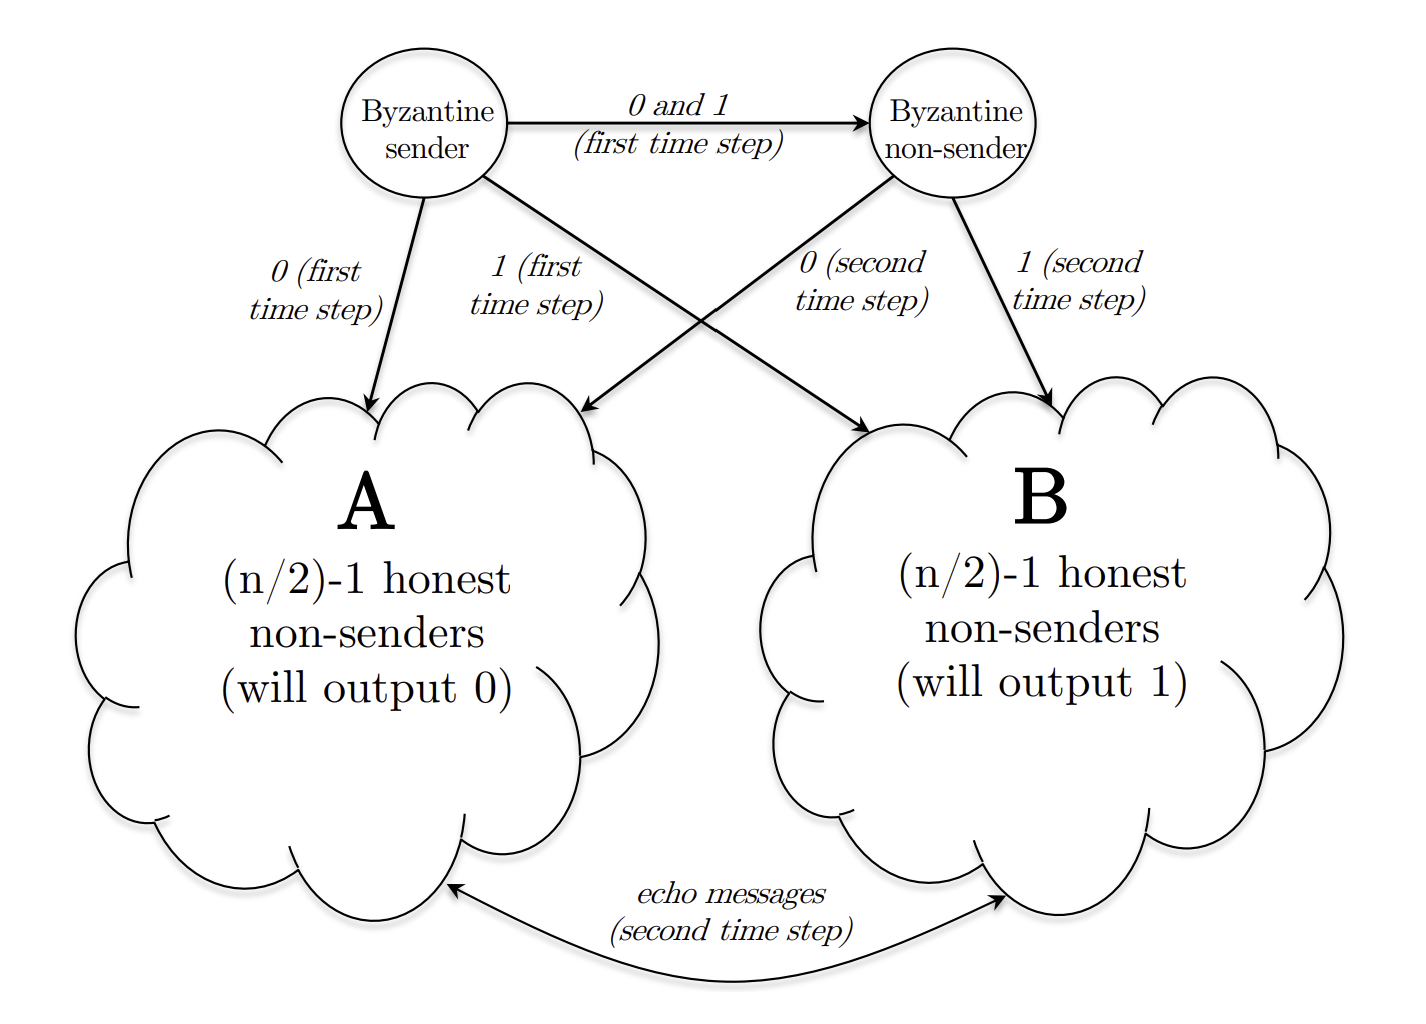
\includegraphics[scale = 0.5]{figures/f2.png}
    \caption{Illustration of a coordinated Byzantine strategy with $f = 2$. Whenever
a node sends or echoes a message, it adds its own signature.}
    \label{fig:mesh1}
\end{figure}\\
Thus, each of the Byzantine nodes uses the canonical ploy of sending conflicting messages to
different honest nodes. The second step above defeats the PKI assumption and enables the
Byzantine non-sender to use such a strategy.
What do the honest non-senders output in the third time step? In the second time step,
each node of A will hear $\frac{n}{2}$ votes for ”0” (one from the sender, $\frac{n}{2} - 2$ from the other
nodes of A, and the tie-breaking vote from the Byzantine non-sender) and $(\frac{n}{2}) - 1$ votes
for “1” (from the nodes of B). Each such node will therefore output “0”. Similarly, each
node of B will output “1”, violating agreement.\\
Three takeaways from this bad example:
\begin{enumerate}
    \item Many seemingly good protocols are not robust to Byzantine faults, in large part because
Byzantine nodes effectively have the power to fully coordinate their deviations from
the intended protocol.
    \item Even when a protocol is robust to Byzantine faults, the rich space of coordinated
Byzantine strategies can make it difficult to rigorously prove it.
    \item It would seem with more than one Byzantine node, more than one round of crosschecking is necessary. This is exactly what happens in the Dolev-Strong protocol in
the next section, in which every additional round of cross-checking enables robustness
to one additional Byzantine node.
\end{enumerate}


\section{The Dolev-Strong Protocol}
This section describes a classic (from 1983) solution to the Byzantine broadcast problem (in
the permissioned and synchronous setting, and assuming PKI), due to Dolev and Strong [2]. 
Coupled with the reduction in Section 2.6, this protocol gives a solution to the state machine
replication problem (under the same assumptions).\\
\subsection{Motivation}
Full disclosure: you’re not going to see the Dolev-Strong protocol mentioned very frequently
in blockchain whitepapers and discussions. One reason for this is the protocol’s heavy reliance
on the synchronous model, which is an overly simplistic model of a global communication
network like the Internet. A second issue is that the protocol always requires a number of
time steps linear in $f$ (the maximum-possible number of Byzantine nodes), which is more
than one would like.\\
Nevertheless, there are several reasons to spend some quality time with the Dolev-Strong
protocol:
\begin{enumerate}
    \item It’s one of the greatest hits of distributed computing. Just as it’s satisfying to experience first-hand famous works of art, so too with famous algorithms and proofs in
computer science.
    \item It doesn’t take that long. The protocol description is short, and the proofs of agreement
and validity are clever but also short.
    \item It would be pedagogically unsound to jump straight into the relatively complicated
consensus protocols that form the basis of actual real-world blockchain protocols. Better to gradually ramp up the difficulty of the setting and the complexity of solutions.
After spending some time getting comfortable in the relatively safe confines of the
synchronous model, we can climb the next mountaintop and design consensus protocols that work well even under much weaker assumptions about the communication
network.
\end{enumerate}

\subsection{Convincing Messages}
We need one definition before proceeding to the description of the Dolev-Strong protocol.
To motivate it, recall that in the simple cross-checking protocol in Section 2.7, non-senders
compare notes in an attempt to pool together all the messages that the (possibly Byzantine)
sender sent out in the first step—if any two of the messages sent differ, then the nonsenders can safely conclude that the sender is Byzantine, stop worrying about the validity
requirement, and achieve agreement by all outputting some canonical value (e.g., the empty
list of transactions). (And as we saw in Section 2.9, such pooling can be tricky to pull off
if there are Byzantine non-senders acting in cahoots with a Byzantine sender) The next
definition establishes conditions under which an honest non-sender can accurately conclude
that a particular message was indeed sent by the sender to some node in the first time step.
(For convenience, for the rest of this lecture we number the time steps starting from 0.)

\dfn{Convincing Messages}{A node $i$ is convinced of value $v$ at time step $t$
if it receives a message prior to that time step that:
\begin{itemize}
    \item references the value $v$;
    \item is signed first by the sender;
    \item is signed also by at least $t - 1$ other distinct nodes, none of which are i.
For example, if node 7 receives at time step 3 a message with a vote for “0” that is signed
first by the sender (node 17, say) and also by nodes 23 and 29, then node 7 is convinced of
the value 0 by this message.
\end{itemize}
}

\subsection{Protocol Description}
Here, finally, is the description of the Dolev-Strong protocol (i.e., the instructions carried
out by honest nodes):

\nt{
\begin{center}
    \textbf{The Dolev-Strong Protocol}
\end{center}
\textbf{Time step 0:} the sender sends its private input $v^*$
(with its signature
attached) to all the non-senders, and outputs $v^*$.\\
\textbf{Time step $t = 1, 2, \cdots, f + 1$:} if a non-sender $i$ is convinced of a value $v$
by a message $m$ received prior to this time step and had not previously been
convinced of $v$, the node adds its own signature to m and sends the resulting
signed message $(m, s)$ to all other non-senders.\\
\textbf{Final output:} for each non-sender, if it is convinced of exactly one value $v$,
it outputs $v$. Otherwise (having detected a Byzantine sender), it outputs $\bot$.}


The symbol $\bot$ denotes some canonical value, such as the empty list of transactions. As
usual, $f$ denotes the maximum number of nodes that might be Byzantine. Recall that its
value is known up front, and indeed the protocol description replies on that knowledge.
The protocol obviously makes use of the PKI assumption (so that nodes can verify each
other’s signatures), and our analysis of it in Section 2.10 will depend crucially on the reliable
communication promised by the synchronous model.\\
Intuitively, time steps after the first one, represent the multiple rounds of cross-checking, with
each (honest) non-sender telling the world about any values that its newly convinced of.
Each non-sender is trying to catch a possible Byzantine sender red-handed by looking for
contradictory messages sent out by the sender at time step 0.\\
Don’t let the brevity of the protocol description fool you, it’s really quite clever. This
should be come clear to you in the next section, where we’ll see short and sweet proofs that
the protocol satisfies both validity and agreement (in the synchronous model), no matter
how many of the nodes are Byzantine.

\section{Properties of the Dolev-Strong Protocol}
This section proves that, under assumptions 1–3 of Section 2.2, the Dolev-Strong protocol
is a solution to the Byzantine broadcast problem: it satisfies termination, validity, and
agreement. Termination is obvious from the protocol description. Let’s see why the other two
properties hold, as well.
\thm{Validity of the Dolev-Strong Protocol}{\textit{Under assumptions 1–3 of
Section 2.2, the Dolev-Strong protocol satisfies validity.}\\
\begin{myproof}
Assume that the sender is honest (as otherwise validity holds vacuously), with private
value $v^*$. Thus, the sender follows the protocol, sending out signed copies of $v^*$
to all the
non-senders at time step 0 and then terminating immediately. Because signatures can’t be forged (by our standing ideal signatures assumption) and no one other than the sender knows
the sender’s private key, there will never be any other messages that include the sender’s
signature. Looking at the second criterion of convincing messages (Definition 2.9.1), we can
conclude that no honest non-sender will ever be convinced of any value other than $v^*$. Are we done? Not quite. The worry is that some honest non-senders might get convinced
of nothing (and thus output $\bot$, rather than $v^*$
). This worried is unfounded. Because the
sender is honest, it sends out signed copies of $v^*$
to all non-senders at time step 0. Because
we’re working in the synchronous model, all of these messages will be received by their
recipients before the start of time step $t = 1$. These messages satisfy Definition 10.1—
because $t = 1$, no signatures other the sender’s are required—and so all honest non-senders
are convinced of $v^*$ already in time step $t = 1$. The only messages in circulation for the entire protocol are the ones signed by the sender, all of which reference to the same value $v^*$. So, it's impossible to convince an honest node by any other value than $v^*$ because the sender never sent any message with another value and noone else can forge a message from the sender with that value.
\end{myproof}
}
\thm{Agreement of the Dolev-Strong Protocol}{\textit{Under assumptions 1–3 of
Section 2.2, the Dolev-Strong protocol satisfies agreement.}\\
\begin{myproof}
Assume that the sender is Byzantine (validity already implies agreement for the
special case of an honest sender). The plan is to prove that, when the protocol terminates,
all honest non-senders have been convinced of exactly the same set of values. If true, this
would imply agreement. The honest non-senders are either all convinced of the same single
value $v$ (in which case they all output $v$), the same set of 2 or more values (in which case
they all output ⊥), or of no values at all (ditto).
So, suppose that an honest non-sender $i$ gets newly convinced of a value $v$ by a message m
received before the start of a time step $t$. We need to show that all other honest non-senders
also get convinced of $v$ before the end of the protocol.\\

\noindent
\textbf{Case 1:} $t \leq f$. In this case, the timer has not yet gone off and $i$ still has time to tell
its colleagues about $v$. Precisely, because $i$ is honest, it follows the protocol and adds its
own signature to $m$ and sends the resulting signed message $(m, s)$ to all other non-senders.
Because we’re working in the synchronous model, every other honest non-sender $j$ receive
this message prior to the start of time step $t + 1$. The signed message $(m, s)$ is signed
first by the sender (because $m$ was signed first by the sender) and also by at least $t$ other
distinct nodes (because $m$ was signed by at least $t - 1$ other distinct nodes, none of which
were $i$). If $(m, s)$ includes $j$’s signature, then $j$ must have been convinced of $v$ at some earlier
point in time (honest non-senders only add their signatures to newly convincing messages).
Otherwise, because $(m, s)$ satisfies the criteria of Definition 2.9.1, $j$ becomes convinced of $v$
at time step $t + 1$.\\

\noindent
\textbf{Case 2:} $t = f + 1$. In this case, $i$ becomes convinced of $v$ only as the game clock expires.
There is no time for $i$ to notify its honest non-sender colleagues about its new conviction,
so the only hope is that $i$ is late to the party and that everyone else independently became
convinced of $v$ (perhaps at time step $f + 1$, or perhaps earlier). Next we’ll see that the
Dolev-Strong protocol uses as many rounds as it does exactly so that this hope is in fact
true.\\
For node $i$ to become convinced of $v$ for the first time at time step $f + 1$, according to
Definition 2.9.1, it must have received a message $m$ with $v$ and signatures from at least $f + 1$
different nodes (one from the sender and at least $t - 1 = f$ from non-senders). Because at
most $f$ of the nodes are Byzantine (by assumption), at least one of these signatures must have
been contributed by an honest (non-sender) node (node $j$, say). Because $i$ received $m$ prior
to the start of time step $f + 1$, $j$ contributed its signature at some earlier time step $t^{'} \leq f$.
(If you think about it, $t^{'}$ must equal $f$) Whenever an honest non-sender adds a signature
to a message, it broadcasts it to all other non-senders. The argument in Case 1 now applies
(with $j$ playing the role of $i$)-$i$ didn't have time to notify all the other honest non-senders,
but $j$ did. Thus, every honest non-sender is convinced of $v$ by time step $t^{'} + 1 \leq f + 1$.
\end{myproof}
}
\qs{}{A good homework exercise is to convince yourself that Theorem 2.10.2 no longer holds if
you stop the protocol one round early, after time step $f$ rather than time step $f + 1$. (What
would be the strategy for the Byzantine nodes?)}

\newpage
\section{ Discussion: How Big Can $f$ Be?}
Let’s conclude by observing a very unusual property of the Dolev-Strong protocol with
respect to the assumed upper bound $f$ on the number of Byzantine nodes. As we noted, the
protocol description depends on $f$, and the protocol’s running time depends linearly on $f$.
Maybe this isn't surprising—the more Byzantine nodes, the more challenging the problem
and the harder we expect to work. But does the protocol ever stop being correct?
Re-reading the proofs of Theorems 2.10.1 and 2.10.2, we see that both work no matter what $f$
is. This is very unusual in distributed computing, and we won’t see another result like it.
Much more commonly, protocols become incorrect (and sometimes consensus problems even
become unsolvable) once $f$ crosses a certain threshold, such as $\frac{n}{3}$ or $\frac{n}{2}$.\\

\noindent
\textbf{Back to SMR.} We should remember the reason that we studied the Byzantine broadcast problem: Protocols that solve it can be used as a subroutine (along with rotating leaders) to solve the problem that we really care about, state machine replication (Section 2.6). Combining the
properties of this reduction (Theorem 2.6.1) with the guarantees of the Dolev-Strong protocol
(Theorems 2.10.1 and 2.10.2) shows that the resulting SMR protocol satisfies consistency and
liveness, no matter what $f$ is.
Many applications of SMR only make sense, however, when there’s an honest majority
(i.e., when $f \leq n/2$). Imagine each node is maintaining a copy of a database, or a copy
of a blockchain. Think of a client who want to run a database query or check the current
cryptocurrency balance of an account. By consistency, all honest nodes will respond to such
a query with the exact same (correct) answer. Byzantine nodes might well lie and respond
to such a query arbitrarily. If a strict majority of the nodes are honest, a user can send their
query to all the nodes and take a majority vote of their answers to determine the correct one. If there’s a 50/50 split of honest and Byzantine nodes, with the latter coordinating on
a fabricated alternative state of the database or blockchain, a client cannot know whom to
believe.\\

\noindent
\textbf{Looking ahead.} Nodes running the Dolev-Strong protocol are contributing and verifying
digital signatures all over the place, crucially relying on the PKI assumption. Could there
be a different protocol for Byzantine broadcast that is equally fault-tolerant but does not
require in-advance distribution of nodes’ public keys? Next lecture is our first impossibility
result: a “hexagon proof” that shows that the answer is “no.” The existence of public-key
cryptography and the ability to carry out a trusted setup really matter!


